% !TeX root = ../main.tex

\chapter{Folgen und Konvergenz}\label{chap:Folgen und Konvergenz} % (fold)
\section{Folgen}

\dfn{Folge} {
  Eine Folge in $\bbK(\bbQ, \bbR)$ ist eine Abbildung von $\bbN \to \bbK$. \\
  Jedem $n \in \bbN$ wird eine Zahl $a_n \in \bbK$ zugeordnet.
}
\ex{Folge} {
  \begin{enumerate}
    \item $a_n = n \cdot \frac1n$ konstante Folge
    \item $a_n = \frac1n$
    \item $a_n = \begin{cases}
        n, &\text{ falls } n \text{ ungerade}\\
        \frac1n &\text{ falls } n \text{ gerade}
      \end{cases}$
    \item Rekursive Folgen: 
      $a_1 = a$ für ein $a \in \bbR$.
      $$
    a_n = \frac12 \left(a_{n-1} + \frac1{a_{n-1}}\right)
      $$
  \end{enumerate}
}

\thm{Existenz und Eindeutigkeit der Abbildungen \(A_n\)}{
  Sei \(a\in\bbK\) so gewählt, dass die folgende rekursive Definition
  wohldefiniert ist. Für jedes \(n\in\bbN\) existiert genau eine
  Abbildung
  \[
  A_n\colon \{1,\dots,n\}\to\bbK
  \]
  mit
  \[
  A_n(1)=a
  \]
  und
  \[
  A_n(k)=\frac12\left(
  A_n(k-1)+\frac{1}{A_n(k-1)}
  \right)
  \qquad\text{für }2\le k\le n.
  \]
}

\begin{myproof}
  Wir beweisen die Aussage durch vollständige Induktion nach \(n\).

  \textbf{Induktionsanfang:}
  Für \(n=1\) ist
  \[
  A_1\colon\{1\}\to\bbK,\qquad A_1(1)=a.
  \]
  Damit ist \(A_1\) eindeutig bestimmt.

  \textbf{Induktionsvoraussetzung:}
  Sei \(n\ge 2\). Wir nehmen an, dass die Abbildung
  \[
  A_{n-1}\colon\{1,\dots,n-1\}\to\bbK
  \]
  existiert und eindeutig bestimmt ist.

  \textbf{Induktionsschritt:}
  Wir definieren \(A_n\colon\{1,\dots,n\}\to\bbK\) durch
  \[
  A_n(k):=
  \begin{cases}
  A_{n-1}(k),&1\le k\le n-1,\\[4pt]
  \displaystyle
  \frac12\left(
  A_{n-1}(n-1)+\frac{1}{A_{n-1}(n-1)}
  \right),&k=n.
  \end{cases}
  \]
  Für \(k\le n-1\) erfüllt \(A_n\) die gewünschten Eigenschaften
  aufgrund der Induktionsvoraussetzung. Für \(k=n\) erfüllt \(A_n\)
  die Rekursionsgleichung nach Definition.

  Die Abbildung \(A_n\) existiert somit. Sie ist auch eindeutig:
  Die Werte \(A_n(1),\dots,A_n(n-1)\) sind durch die
  Induktionsvoraussetzung eindeutig bestimmt, und der Wert \(A_n(n)\)
  ist durch die Rekursionsgleichung eindeutig festgelegt.

  Damit ist die Aussage für alle \(n\in\bbN\) bewiesen.
  \end{myproof}

Aus dieser Konstruktion ergibt sich unmittelbar die folgende Definition:

\dfn{Die zugehörige Folge}{
  Wir definieren die Folge \((a_n)_{n\in\bbN}\) durch
  \[
  a_n:=A_n(n).
  \]
  Insbesondere gilt
  \[
  a_1=a,\qquad
  a_n=\frac12\left(a_{n-1}+\frac1{a_{n-1}}\right)
  \quad\text{für }n\ge 2.
  \]
}

\nt{
  Damit der Beweis vollständig mathematisch korrekt ist, müssen die Voraussetzungen an \(\bbK\) und \(a\) sicherstellen, dass die Division durch \(A_n(k-1)\) stets möglich ist. Beispielsweise genügt \(\bbK=\bbR\) und \(a>0\).
}

\section{Konvergenz und Beschränktheit}
\dfn{Konvergenz} {
  Eine Folge $a_n$ heißt konvergent gegen $a \in \bbR$ falls es zu jeden $\epsilon > 0$ ein $n(\epsilon) > 0$ mit $\vert A_n - a\vert < \epsilon \forall n \ge n(\epsilon)$ \\
  $$\lim_{n \to \infty} a_n= a$$
}
\ex{} {
  \begin{enumerate}
    \item $a_n  = a = \lim_{n \to \infty} a_n = 1$
    \item $a_n = \frac1n, \lim_{n \to \infty} a_n = 0$, denn zu $\epsilon > 0 $ wähle $n(\epsilon) > \frac1\epsilon \implies \frac1{n(\epsilon)} < \epsilon$ \\
      \begin{align*} 
        \frac1m < \frac1{n(\epsilon)} &< \epsilon &\forall m > n(\epsilon) \\
        \vert \frac1n - 0 \vert &= \frac1n < \epsilon &\text{ für } n \ge n(\epsilon)
      \end{align*}
  \end{enumerate}
}

\dfn{Beschränktheit} {
  Eine Folge heißt \textbf{beschränkt}, falls die Menge $M = {a_n \vert n}$ beschränkt ist.
}
\nt {
  $(a_n)$ ist beschränkt $\Leftrightarrow$ $(\vert a_n \vert)$ ist beschränkt. \\
  Eine Menge ist beschränkt, falls es eine obere und eine untere Schranke gibt.
}
\thm{Beschränktheit konvergenter Folgen}{
  Jede konvergente Folge \((a_n)_{n\in\bbN}\) reeller Zahlen ist
  beschränkt. Das heißt: Ist
  \[
  \lim_{n\to\infty}a_n=a\in\bbR,
  \]
  so existieren \(m,M\in\bbR\) mit
  \[
  m\le a_n\le M
  \qquad\text{für alle }n\in\bbN.
  \]
}

\begin{myproof}
  Sei \(a_n\to a\). Nach Definition der Konvergenz existiert zu
  \(\varepsilon=1\) ein \(n_0\in\bbN\), sodass
  \[
  |a_n-a|<1
  \qquad\text{für alle }n\ge n_0.
  \]
  Daraus folgt
  \[
  a-1<a_n<a+1
  \qquad\text{für alle }n\ge n_0.
  \]

  Die Folgenglieder ab dem Index \(n_0\) sind somit nach oben durch
  \(a+1\) und nach unten durch \(a-1\) beschränkt.

  Die ersten \(n_0-1\) Folgenglieder bilden eine endliche Menge.
  Daher existieren
  \[
  M:=\max\{a_1,\dots,a_{n_0-1},a+1\}
  \]
  und
  \[
  m:=\min\{a_1,\dots,a_{n_0-1},a-1\}.
  \]
  Falls \(n_0=1\), entfallen die endlich vielen Anfangsglieder in
  diesen Mengen, sodass \(M=a+1\) und \(m=a-1\) gewählt werden können.

  Für \(n<n_0\) gilt aufgrund der Definition von \(m\) und \(M\)
  \[
  m\le a_n\le M.
  \]
  Für \(n\ge n_0\) folgt dieselbe Ungleichung aus
  \[
  a-1<a_n<a+1
  \]
  und der Wahl von \(m\) und \(M\).

  Somit gilt insgesamt
  \[
  m\le a_n\le M
  \qquad\text{für alle }n\in\bbN.
  \]
  Also ist die Folge \((a_n)_{n\in\bbN}\) beschränkt.
\end{myproof}

\nt{$(-1)^n$ ist beschränkt, aber nicht konvergent.}

\mlemma{Beschränktheit Absolutbetrag von Folgen} {
  Eine Folge $a$ ist genau dann beschränkt, wenn die Folge $\vert a \vert $ mit Folgengliedern $\vert a_n \vert$ nach oben beschränkt ist.
}

\begin{myproof}
  Wenn die Folge $\vert a \vert$ nach oben beschränkt ist, so ist sowohl $a$ als auch $-a$ nach oben beschränkt, also ist $a$ nach oben und nach unten bschränkt, also ist $a$ beschränkt. Umgekehrt sind, wenn $a$ beschränkt ist, sowohl $a$ als auch $-a$ nach oben beschränkt, und daher $\vert a \vert$ nach oben beschränkt.
\end{myproof}

\section{Konvergente Folgen}

\qs{} {
  Wann konvergiert eine Folge $(a_n)$?
}

\sol Die Folge $(a_n)$ konvergiert gegen $a$, falls
  \[
    \forall \varepsilon > 0\;
    \exists n_0 \in \bbN\;
    \forall n \ge n_0:
    |a_n-a| < \varepsilon.
  \]

  Jede konvergente Folge ist beschränkt.

\begin{theorem}{Konvergente Folgen sind Cauchy-Folgen}{conv-cauchy}
  Jede konvergente Folge ist eine Cauchy-Folge.
\end{theorem}

\begin{myproof}
  Sei $(a_n)$ eine Folge mit $a_n \to a$.

  Für jedes $\varepsilon > 0$ existiert ein $n_0 \in \bbN$,
  sodass für alle $n \ge n_0$ gilt:
  \[
    |a_n-a| < \frac{\varepsilon}{2}.
  \]

  Für alle $n,m \ge n_0$ folgt mit der Dreiecksungleichung:
  \begin{align*}
    |a_n-a_m|
    &= |a_n-a+a-a_m|\\
    &\le |a_n-a|+|a-a_m|\\
    &< \frac{\varepsilon}{2}
       +\frac{\varepsilon}{2}
     = \varepsilon.
  \end{align*}

  Also ist $(a_n)$ eine Cauchy-Folge.
\end{myproof}

\section{Geometrische Folgen}

\ex{Geometrische Folge}{
  Sei
  \[
    a_n=b^n.
  \]

  Für $0<b<1$ ist $(a_n)$ monoton fallend und
  nach unten durch $0$ beschränkt.
}

\thm{Grenzwert einer geometrischen Folge}{
  Für $0<b<1$ gilt
  \[
    \lim_{n\to\infty}b^n=0.
  \]
}

\begin{myproof}
  Da $(b^n)$ monoton fallend und beschränkt ist,
  ist die Folge konvergent. Sei
  \[
    L:=\lim_{n\to\infty}b^n.
  \]

  Definiere $c_n:=a_{n+1}$. Dann gilt
  \[
    \lim_{n\to\infty}c_n
    =\lim_{n\to\infty}a_n=L.
  \]

  Andererseits ist
  \[
    c_n=b\cdot a_n.
  \]
  Mit den Grenzwertsätzen folgt
  \[
    L=\lim_{n\to\infty}c_n
     =b\lim_{n\to\infty}a_n
     =bL.
  \]

  Da $b\ne1$, folgt $L=0$.
\end{myproof}

\section{Algebraische Struktur konvergenter Folgen}

\thm{Ring der konvergenten Folgen}{
  Die Menge der konvergenten Folgen bildet mit
  komponentenweiser Addition und Multiplikation
  einen kommutativen Ring mit Eins.
}

\nt{
  Für konvergente Folgen $(a_n)$ und $(b_n)$
  definieren wir die Operationen durch
  \begin{align*}
    (a_n)+(b_n)&:=(a_n+b_n),\\
    (a_n)\cdot(b_n)&:=(a_nb_n).
  \end{align*}
}

\subsection{Addition}

\begin{myproof}
  Die Assoziativität und Kommutativität der Addition
  folgen aus den entsprechenden Eigenschaften
  der rationalen Zahlen.

  Das neutrale Element ist die konstante Nullfolge
  \[
    (0)=(0,0,0,\dots).
  \]

  Das additive Inverse zu $(a_n)$ ist
  \[
    -(a_n):=(-a_n).
  \]

  Es bleibt zu zeigen, dass die Summe zweier
  konvergenter Folgen wieder konvergiert.

  Seien
  \[
    \lim_{n\to\infty}a_n=a,
    \qquad
    \lim_{n\to\infty}b_n=b.
  \]

  Für jedes $\varepsilon>0$ existieren
  $n_1,n_2\in\bbN$, sodass
  \begin{align*}
    |a_n-a|&<\frac{\varepsilon}{2}
      &&\text{für }n\ge n_1,\\
    |b_n-b|&<\frac{\varepsilon}{2}
      &&\text{für }n\ge n_2.
  \end{align*}

  Setze $n_0:=\max\{n_1,n_2\}$.
  Für alle $n\ge n_0$ gilt:
  \begin{align*}
    |(a_n+b_n)-(a+b)|
    &=|(a_n-a)+(b_n-b)|\\
    &\le |a_n-a|+|b_n-b|\\
    &<\varepsilon.
  \end{align*}

  Also konvergiert $(a_n+b_n)$ gegen $a+b$.
\end{myproof}

\subsection{Multiplikation}

\dfn{Multiplikation von Folgen}{
  Für zwei Folgen $(a_n)$ und $(b_n)$ definieren wir
  \[
    (a_n)\cdot(b_n):=(a_nb_n).
  \]
}

\thm{Grenzwert eines Produkts}{
  Sind $(a_n)$ und $(b_n)$ konvergent mit
  \[
    \lim_{n\to\infty}a_n=a,
    \qquad
    \lim_{n\to\infty}b_n=b,
  \]
  so gilt
  \[
    \lim_{n\to\infty}(a_nb_n)=ab.
  \]
}

\begin{myproof}
  Wir betrachten
  \begin{align*}
    |a_nb_n-ab|
    &=|a_nb_n-ab_n+ab_n-ab|\\
    &=|(a_n-a)b_n+a(b_n-b)|\\
    &\le |a_n-a|\,|b_n|
       +|a|\,|b_n-b|.
  \end{align*}

  Da $(b_n)$ konvergiert, ist die Folge beschränkt.
  Es existiert also $M>0$ mit
  \[
    |b_n|\le M
    \qquad\text{für alle }n\in\bbN.
  \]

  Sei $\varepsilon>0$. Wegen der Konvergenz
  existiert ein $n_0\in\bbN$, sodass für
  alle $n\ge n_0$ gilt:
  \begin{align*}
    |a_n-a|&<\frac{\varepsilon}{2M},\\
    |b_n-b|&<\frac{\varepsilon}{2(|a|+1)}.
  \end{align*}

  Damit folgt
  \begin{align*}
    |a_nb_n-ab|
    &\le M|a_n-a|+|a|\,|b_n-b|\\
    &<\frac{\varepsilon}{2}
      +\frac{|a|}{|a|+1}\frac{\varepsilon}{2}\\
    &\le\varepsilon.
  \end{align*}

  Also konvergiert $(a_nb_n)$ gegen $ab$.
\end{myproof}

\nt{
  Die Distributivgesetze folgen komponentenweise
  aus den Distributivgesetzen in $\bbQ$.

  Das multiplikative neutrale Element ist
  die konstante Einsfolge
  \[
    (1)=(1,1,1,\dots).
  \]

  Somit bilden die konvergenten rationalen Folgen
  mit den definierten Operationen einen
  kommutativen Ring mit Eins.
}

\thm{Grenzwertabbildung als Ringhomomorphismus}{
  Die Abbildung
  \[
    \varphi\colon (a_n)\longmapsto
    \lim_{n\to\infty}a_n
  \]
  ist ein Ringhomomorphismus von der Menge
  der konvergenten rationalen Folgen nach $\bbQ$.
}

\begin{myproof}
  Für zwei konvergente Folgen $(a_n)$ und $(b_n)$
  gelten die Grenzwertsätze:
  \begin{align*}
    \varphi((a_n)+(b_n))
    &=\lim_{n\to\infty}(a_n+b_n)\\
    &=\lim_{n\to\infty}a_n
      +\lim_{n\to\infty}b_n\\
    &=\varphi((a_n))+\varphi((b_n)),
  \end{align*}
  sowie
  \begin{align*}
    \varphi((a_n)\cdot(b_n))
    &=\lim_{n\to\infty}(a_nb_n)\\
    &=\lim_{n\to\infty}a_n
      \cdot\lim_{n\to\infty}b_n\\
    &=\varphi((a_n))\cdot\varphi((b_n)).
  \end{align*}

  Außerdem gilt $\varphi((1))=1$.
  Damit ist $\varphi$ ein Ringhomomorphismus.
\end{myproof}

\section{Cauchy-Folgen}
\begin{definition}{Cauchy-Folgen}{cauchy}
  Eine Folge $a$ von rationalen Zahlen heißt \textbf{Cauchy-Folge},genau dann wenn folgendes gilt:
  $$
    \forall k \in \bbN \exists n_0 \in \bbN \forall n \ge n_0 \forall m \ge n_0: \vert a_n - a_m \vert \le \frac1k
    $$
\end{definition}

Diese komplizierte Definition besagrt einfach, dass sich fast alle Folgenglieder $a_n$ sich kaum mehr von $a_n$ unterscheiden werden.

\nt {
  Mit Hilfe der Dreiecksungleichung kann man leicht zeigen, dass eine Folge Cauchy-Folge ist, wenn
  $$
    \forall k \in \bbN \exists n \in \bbN \forall m \ge 0: \vert a_n - a_{n + m} \le \frac1k
  $$
}
\begin{figure}[htbp]
    \centering
    \resizebox{\textwidth}{!}{
      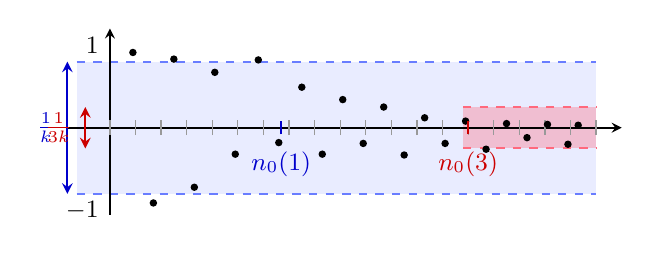
\begin{tikzpicture}[
          x=0.65cm,
          y=1.05cm,
          >=stealth,
          every node/.style={font=\small}
      ]

      % Colors
      \definecolor{lightblue}{RGB}{105,125,255}
      \definecolor{lightred}{RGB}{255,105,125}

      % Blue interval (the 1/k-wide "tube")
      \fill[lightblue,opacity=0.15]
          (-0.65,-0.8) rectangle (9.5,0.8);

      \draw[lightblue,dashed,line width=0.7pt]
          (-0.65,0.8) -- (9.5,0.8);
      \draw[lightblue,dashed,line width=0.7pt]
          (-0.65,-0.8) -- (9.5,-0.8);

      % Red interval around n_0(3)
      \fill[lightred,opacity=0.35]
          (6.9,-0.25) rectangle (9.5,0.25);

      \draw[lightred,dashed,line width=0.7pt]
          (6.9,-0.25) -- (9.5,-0.25);
      \draw[lightred,dashed,line width=0.7pt]
          (6.9,0.25) -- (9.5,0.25);

      % Axes
      \draw[->,line width=0.6pt]
          (-0.85,0) -- (10,0);
      \draw[->,line width=0.6pt]
          (0, -1.05) -- (0,1.2);

      % Axis labels
      \node[left] at (-0.03,1) {$1$};
      \node[left] at (-0.03,-1) {$-1$};

      % Horizontal ticks
      \foreach \x in {-0.5,0.0,...,9.5} {
          \draw[gray!80,line width=0.45pt]
              (\x,-0.09) -- (\x,0.09);
      }

      % Points above and below the axis
      \foreach \x/\y in {
          0.45/0.91,
          1.25/0.83,
          2.05/0.67,
          2.9/0.82,
          3.75/0.49,
          4.55/0.34,
          5.35/0.25,
          6.15/0.12,
          6.95/0.08,
          7.75/0.05,
          8.55/0.04,
          9.15/0.03,
          0.85/-0.91,
          1.65/-0.72,
          2.45/-0.32,
          3.3/-0.18,
          4.15/-0.32,
          4.95/-0.19,
          5.75/-0.33,
          6.55/-0.19,
          7.35/-0.26,
          8.15/-0.12,
          8.95/-0.20
      } {
          \fill (\x,\y) circle (1.35pt);
      }

      % Markers for n_0(1) and n_0(3)
      \draw[blue!80!black,line width=0.7pt]
          (3.35,-0.08) -- (3.35,0.08);
      \node[blue!80!black,below=5pt] at (3.35,0)
          {$n_0(1)$};

      \draw[red!80!black,line width=0.7pt]
          (7.0,-0.08) -- (7.0,0.08);
      \node[red!80!black,below=5pt] at (7.0,0)
          {$n_0(3)$};

      % Width annotations on the left
      \draw[<->,blue!80!black,line width=0.7pt]
          (-0.83,-0.8) -- (-0.83,0.8);
      \node[blue!80!black,left=1pt] at (-0.83,0)
          {$\frac{1}{k}$};

      \draw[<->,red!80!black,line width=0.7pt]
          (-0.48,-0.25) -- (-0.48,0.25);
      \node[red!80!black,left=1pt] at (-0.48,0)
          {$\frac{1}{3k}$};

      \end{tikzpicture}
    }
    \caption{Beispiel einer Cauchy-Folge. Ab einem $n_0$,
    das von $k\in\bbN$ abhängt, liegen alle Folgenglieder
    in einem $\frac{1}{k}$-weiten "Schlauch".}
    \label{fig:cauchy-schlauch}
\end{figure}

\begin{figure}[htbp]
    \centering
    \resizebox{\textwidth}{!}{%
    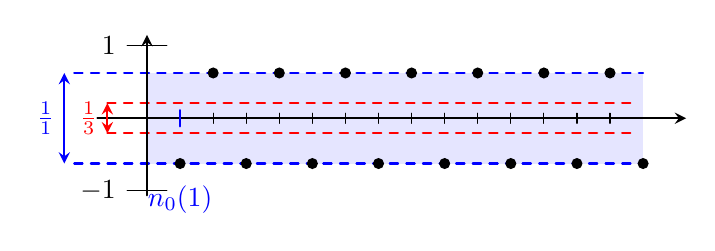
\begin{tikzpicture}[
        x=0.42cm,
        y=1.15cm,
        >=stealth,
        line cap=round
    ]

    % Shaded band
    \fill[blue!10] (0,-0.5) rectangle (15,0.5);

    % Blue dashed boundaries
    \draw[blue,dashed,thick] (-2.2,0.5) -- (15,0.5);
    \draw[blue,dashed,thick] (-2.2,-0.5) -- (15,-0.5);

    % Red comparison band: width 1/3
    \draw[red,dashed,thick] (-1.2,1/6) -- (14.7,1/6);
    \draw[red,dashed,thick] (-1.2,-1/6) -- (14.7,-1/6);

    % Axes
    \draw[->,thick] (-1.5,0) -- (16.3,0);
    \draw[->,thick] (0,-0.85) -- (0,0.92);

    % Vertical axis ticks and labels
    \draw ( -0.6,0.8) -- (0.6,0.8);
    \draw ( -0.6,-0.8) -- (0.6,-0.8);
    \node[left] at (-0.65,0.8) {$1$};
    \node[left] at (-0.65,-0.8) {$-1$};

    % Horizontal axis ticks
    \foreach \x in {1,...,14} {
        \draw (\x,-0.055) -- (\x,0.055);
    }

    % Alternating sequence values +1/2 and -1/2
    \foreach \x in {2,4,...,14} {
        \fill (\x,0.5) circle (2pt);
    }
    \foreach \x in {1,3,...,15} {
        \fill (\x,-0.5) circle (2pt);
    }

    % n_0(1) marker
    \draw[blue,thick] (1, -0.09) -- (1,0.09);
    \node[blue] at (1,-0.9) {$n_0(1)$};

    % Blue width annotation: 1
    \draw[blue,<->,thick] (-2.5,-0.5) -- (-2.5,0.5);
    \node[blue,left] at (-2.5,0) {$\frac{1}{1}$};

    % Red width annotation: 1/3
    \draw[red,<->,thick] (-1.2,-1/6) -- (-1.2,1/6);
    \node[red,left] at (-1.2,0) {$\frac{1}{3}$};

    \end{tikzpicture}%
    }
    \caption{Die Folge mit Folgenglieder $a_n=(-1)^n\frac{1}{2}$
    ist keine Cauchy-Folge. Es gibt kein $n_0$, so dass für alle
    $n\geq n_0$ und alle $m\in\mathbb{N}$ gilt, dass
    $|a_n-a_{n+m}|\leq\frac{1}{3}$.}
    \label{fig:keine-cauchy-folge}
\end{figure}

\nt{
  Eine Cauchy-Folge, dessen Folgenglieder rational sind, nennen wir auch eine rationale Cauchy-Folge.
}

\thm{Beschränktheit von Cauchy-Folgen}{
  Jede Cauchy-Folge ist beschränkt.
}
\begin{myproof}
  Wähle \(k=10\). Sei \(n_0\) die zugehörige Zahl aus der
  Cauchy-Bedingung \Cref{def:cauchy}. Die endlich vielen Zahlen
  \(\lvert a_1\rvert,\lvert a_2\rvert,\dots,\lvert a_{n_0}\rvert\)
  haben einen maximalen Wert
  \[
    M:=\max\{\lvert a_1\rvert,\lvert a_2\rvert,\dots,
    \lvert a_{n_0}\rvert\}.
  \]
  Andererseits gilt für alle \(m\in\bbN\):
  \[
    \lvert a_{n_0}-a_{n_0+m}\rvert\le\frac1{10}.
  \]
  Wegen der Dreiecksungleichung folgt
  \[
    \lvert a_{n_0+m}\rvert
    \le \lvert a_{n_0}\rvert+\frac1{10}
    \le M+\frac1{10}.
  \]
  Daher sind alle Folgenglieder durch \(M+\frac1{10}\) beschränkt.
\end{myproof}

Die Folge \(a_n=\frac1n\) ist offenbar eine Cauchy-Folge, denn für
alle \(m\ge 0\) gilt
\[
  \left\lvert\frac1n-\frac1{n+m}\right\rvert\le\frac1n.
\]
Für jedes \(k\in\bbN\) ist die Cauchy-Bedingung somit beispielsweise
mit \(n_0=k\) erfüllt. Da sich \(\frac1n\) zunehmend der Zahl \(0\)
annähert, lässt sich dies mit dem Begriff der Konvergenz formal
beschreiben.

\dfn{Konvergenz von Folgen}{ 
  Eine Folge \(a\) rationaler Zahlen heißt konvergent in \(\bbQ\),
  falls es eine Zahl \(q\in\bbQ\) gibt, sodass
  \[
    \forall k\in\bbN\ \exists n_0\in\bbN\
    \forall n\ge n_0:
    \lvert a_n-q\rvert\le\frac1k.
  \]
}
Die Zahl \(q\) heißt der \textbf{Grenzwert} oder \textbf{Limes} der
Folge \(a\). Wir schreiben \(\lim a=q\) oder \(a\to q\).

Man prüft leicht nach, dass die Folge mit Folgengliedern
\(a_n=\frac1n\) gegen \(0\) konvergiert. Folgen, die gegen den
Grenzwert \(0\) konvergieren, bezeichnen wir als \textbf{Nullfolgen}.

\thm{Konvergente Folgen sind Cauchy-Folgen}{
  \Cref{th:conv-cauchy}
}

\section{Teilfolgen}

\dfn{Monotone Folgen}{
  Eine Folge $(a_n)$ heißt \textbf{monoton wachsend}, falls
  \[
    \forall n\in\bbN:\quad a_{n+1}\ge a_n.
  \]
  Sie heißt \textbf{streng monoton wachsend}, falls
  \[
    \forall n\in\bbN:\quad a_{n+1}>a_n.
  \]
  Analog definiert man monoton fallende und streng monoton
  fallende Folgen.
}

\nt{
  Statt monoton wachsend sagt man auch \textbf{nicht fallend}.
}

\dfn{Teilfolge}{
  Sei $k\colon\bbN\to\bbN$ eine streng monoton wachsende Folge
  natürlicher Zahlen und sei $a$ eine Folge.

  Dann heißt
  \[
    b:=a\circ k
  \]
  eine \textbf{Teilfolge} oder \textbf{Unterfolge} von $a$.
  Ihre Folgenglieder sind
  \[
    b_n=a_{k_n}.
  \]
}

\mlemma{Teilfolgen von Cauchy-Folgen}{
  Ist $a$ eine Cauchy-Folge und $b$ eine Teilfolge von $a$,
  dann gilt
  \[
    a\sim b.
  \]
  Insbesondere gilt
  \[
    \lim b=\lim a.
  \]
}

\begin{myproof}
  Sei $b_n=a_{k_n}$ eine Teilfolge von $a$.
  Da $(k_n)$ streng monoton wächst, gilt $k_n\ge n$.

  Weil $a$ eine Cauchy-Folge ist, existiert für jedes
  $\varepsilon>0$ ein $n_0\in\bbN$, sodass
  \[
    |a_n-a_m|<\varepsilon
    \qquad\forall n,m\ge n_0.
  \]

  Für alle $n\ge n_0$ gilt insbesondere $k_n\ge n_0$.
  Somit folgt
  \[
    |a_n-b_n|
    =|a_n-a_{k_n}|<\varepsilon.
  \]

  Also ist $(a_n-b_n)$ eine Nullfolge und damit
  $a\sim b$. Folglich besitzen beide Folgen denselben
  Grenzwert.
\end{myproof}

\mlemma{Monotone Unterfolgen}{
  Jede Folge besitzt eine monoton wachsende oder eine
  monoton fallende Teilfolge.
}

\begin{myproof}
  Wir nennen $r\in\bbN$ einen \textbf{Rekord} von $a$, falls
  \[
    \forall m>r:\quad a_m\le a_r.
  \]

  \textbf{Fall 1:} Es gibt unendlich viele Rekorde.

  Dann existiert eine streng monoton wachsende Folge
  $(r_k)$ von Rekordindizes.

  Die Teilfolge $b_k:=a_{r_k}$ ist monoton fallend,
  denn für $r_{k+1}>r_k$ gilt
  \[
    a_{r_{k+1}}\le a_{r_k}.
  \]

  \textbf{Fall 2:} Es gibt nur endlich viele Rekorde.

  Wähle $m_1$ größer als alle Rekordindizes.
  Da $m_1$ kein Rekord ist, existiert $m_2>m_1$ mit
  \[
    a_{m_2}>a_{m_1}.
  \]

  Auch $m_2$ ist kein Rekord. Induktiv erhalten wir
  eine streng monoton wachsende Indexfolge $(m_k)$ mit
  \[
    a_{m_{k+1}}>a_{m_k}.
  \]

  Somit ist $b_k:=a_{m_k}$ eine monoton wachsende
  Teilfolge.

  In beiden Fällen existiert also eine monotone Teilfolge.
\end{myproof}


\section{Konvergenz und Häufungspunkte}

\mlemma{Monotone Konvergenz}{
  Sei $(a_n)$ eine monoton wachsende, beschränkte Folge
  reeller Zahlen. Dann gilt
  \[
    \lim_{n\to\infty}a_n
    =\sup\{a_n:n\in\bbN\}.
  \]

  Entsprechend konvergiert jede monoton fallende,
  beschränkte Folge gegen
  \[
    \inf\{a_n:n\in\bbN\}.
  \]
}

\begin{myproof}
  Sei
  \[
    A:=\{a_n:n\in\bbN\}.
  \]
  Da $A$ nach oben beschränkt ist, existiert
  $s:=\sup A\in\bbR$.

  Nach der Definition des Supremums existiert für jedes
  $\varepsilon>0$ ein $n_0\in\bbN$, sodass
  \[
    a_{n_0}>s-\varepsilon.
  \]

  Wegen der Monotonie gilt für alle $n\ge n_0$:
  \[
    s-\varepsilon<a_n\le s.
  \]

  Also folgt
  \[
    |a_n-s|<\varepsilon.
  \]

  Damit konvergiert $(a_n)$ gegen $s$.
  Der Fall einer monoton fallenden Folge ist analog.
\end{myproof}

\thm{Bolzano--Weierstraß}{
  Jede beschränkte Folge reeller Zahlen besitzt mindestens
  eine konvergente Teilfolge.
}

\begin{myproof}
  Nach dem Lemma über monotone Unterfolgen besitzt jede
  Folge eine monoton wachsende oder monoton fallende
  Teilfolge.

  Da die ursprüngliche Folge beschränkt ist, ist auch
  jede ihrer Teilfolgen beschränkt.

  Nach dem Lemma über monotone Konvergenz konvergiert
  jede beschränkte monotone Folge.

  Also besitzt die ursprüngliche Folge eine konvergente
  Teilfolge.
\end{myproof}


\section{Limes superior und Limes inferior}

\dfn{Limes superior und Limes inferior}{
  Sei $(a_n)$ eine reelle Folge.

  Der \textbf{Limes superior} ist durch
  \[
    \limsup_{n\to\infty}a_n=z
  \]
  charakterisiert, falls
  \begin{align*}
    &\forall k\in\bbN\;
      \exists n_0\in\bbN\;
      \forall n\ge n_0:
      a_n\le z+\frac1k,
    \\
    &\forall k\in\bbN\;
      \forall n_0\in\bbN\;
      \exists n\ge n_0:
      a_n>z-\frac1k.
  \end{align*}

  Entsprechend ist der \textbf{Limes inferior} durch
  \[
    \liminf_{n\to\infty}a_n=y
  \]
  charakterisiert, falls
  \begin{align*}
    &\forall k\in\bbN\;
      \exists n_0\in\bbN\;
      \forall n\ge n_0:
      a_n\ge y-\frac1k,
    \\
    &\forall k\in\bbN\;
      \forall n_0\in\bbN\;
      \exists n\ge n_0:
      a_n<y+\frac1k.
  \end{align*}
}

\nt{
  Der Limes superior beschreibt die kleinste langfristige
  obere Schranke einer Folge, der Limes inferior die
  größte langfristige untere Schranke.
}


\section{Häufungspunkte}

\dfn{Häufungspunkt}{
  Sei $(a_n)$ eine Folge reeller Zahlen.

  Ein Punkt $x\in\bbR$ heißt \textbf{Häufungspunkt} von
  $(a_n)$, falls eine Teilfolge $(a_{n_k})$ existiert mit
  \[
    \lim_{k\to\infty}a_{n_k}=x.
  \]
}

\mlemma{Charakterisierung von Häufungspunkten}{
  Ein Punkt $x\in\bbR$ ist genau dann Häufungspunkt
  einer Folge $(a_n)$, wenn für jedes $k\in\bbN$
  eine unendliche Menge $N_k\subseteq\bbN$ existiert,
  sodass
  \[
    \forall n\in N_k:\quad
    |a_n-x|\le\frac1k.
  \]
}

\begin{myproof}
  \textbf{Hinrichtung:}

  Sei $x$ Häufungspunkt von $(a_n)$. Dann existiert
  eine Teilfolge $(a_{n_j})$, die gegen $x$ konvergiert.

  Für jedes $k\in\bbN$ gibt es einen Index $j_0$,
  sodass für alle $j\ge j_0$ gilt:
  \[
    |a_{n_j}-x|\le\frac1k.
  \]

  Die Menge
  \[
    N_k:=\{n_j:j\ge j_0\}
  \]
  ist unendlich und erfüllt die Behauptung.

  \medskip
  \textbf{Rückrichtung:}

  Angenommen, für jedes $k\in\bbN$ existiert eine
  unendliche Menge $N_k\subseteq\bbN$ mit
  \[
    \forall n\in N_k:\quad
    |a_n-x|\le\frac1k.
  \]

  Wähle $n_1\in N_1$ und anschließend induktiv
  \[
    n_{k+1}\in N_{k+1},
    \qquad n_{k+1}>n_k.
  \]

  Da jedes $N_k$ unendlich ist, ist diese Wahl möglich.

  Damit ist $(n_k)$ streng monoton wachsend, und es gilt
  \[
    |a_{n_k}-x|\le\frac1k.
  \]

  Folglich konvergiert die Teilfolge $(a_{n_k})$
  gegen $x$. Somit ist $x$ ein Häufungspunkt.
\end{myproof}


\mlemma{Limes superior und Häufungspunkte}{
  Sei $(a_n)$ eine reelle Folge.

  Falls
  \[
    \limsup_{n\to\infty}a_n=z\in\bbR,
  \]
  dann ist $z$ der größte Häufungspunkt von $(a_n)$.

  Falls
  \[
    \liminf_{n\to\infty}a_n=y\in\bbR,
  \]
  dann ist $y$ der kleinste Häufungspunkt von $(a_n)$.
}

\begin{myproof}
  Sei
  \[
    z:=\limsup_{n\to\infty}a_n.
  \]

  Zunächst zeigen wir, dass $z$ ein Häufungspunkt ist.

  Nach der Definition des Limes superior existiert
  für jedes $k\in\bbN$ ein $N_k\in\bbN$, sodass
  \[
    a_n\le z+\frac1k
    \qquad\forall n\ge N_k.
  \]

  Außerdem existiert für jedes $n_0\in\bbN$ ein
  $n\ge n_0$ mit
  \[
    a_n>z-\frac1k.
  \]

  Wir wählen induktiv eine streng wachsende Indexfolge
  $(n_k)$, sodass
  \[
    n_k\ge N_k
    \qquad\text{und}\qquad
    a_{n_k}>z-\frac1k.
  \]

  Damit gilt
  \[
    z-\frac1k<a_{n_k}\le z+\frac1k,
  \]
  also
  \[
    |a_{n_k}-z|\le\frac1k.
  \]

  Folglich konvergiert $(a_{n_k})$ gegen $z$.
  Somit ist $z$ ein Häufungspunkt.

  Nun sei $x$ ein beliebiger Häufungspunkt von $(a_n)$.
  Dann existiert eine Teilfolge $(a_{m_k})$ mit
  \[
    a_{m_k}\longrightarrow x.
  \]

  Angenommen, es wäre $x>z$.
  Wähle $\varepsilon>0$ mit
  \[
    2\varepsilon<x-z.
  \]

  Wegen $\limsup a_n=z$ gilt für alle hinreichend
  großen $n$:
  \[
    a_n\le z+\varepsilon.
  \]

  Andererseits gilt wegen $a_{m_k}\to x$
  für alle hinreichend großen $k$:
  \[
    a_{m_k}>x-\varepsilon>z+\varepsilon.
  \]

  Dies ist ein Widerspruch. Also gilt $x\le z$.

  Somit ist $z$ der größte Häufungspunkt.

  Die Aussage für den Limes inferior folgt analog
  durch Umkehrung der Ungleichungen.
\end{myproof}


\mlemma{Konvergenz und Limes superior/inferior}{
  Eine reelle Folge $(a_n)$ konvergiert genau dann
  gegen $x\in\bbR$, wenn
  \[
    \limsup_{n\to\infty}a_n
    =
    \liminf_{n\to\infty}a_n
    =x.
  \]
}

\begin{myproof}
  \textbf{Hinrichtung:}

  Sei $a_n\to x$. Dann existiert für jedes
  $\varepsilon>0$ ein $n_0\in\bbN$, sodass
  für alle $n\ge n_0$ gilt:
  \[
    x-\varepsilon<a_n<x+\varepsilon.
  \]

  Somit erfüllt $x$ sowohl die Bedingungen für den
  Limes superior als auch für den Limes inferior.
  Also gilt
  \[
    \limsup_{n\to\infty}a_n
    =
    \liminf_{n\to\infty}a_n=x.
  \]

  \medskip
  \textbf{Rückrichtung:}

  Sei
  \[
    \limsup_{n\to\infty}a_n
    =
    \liminf_{n\to\infty}a_n=x.
  \]

  Nach der Definition des Limes superior existiert
  für jedes $\varepsilon>0$ ein $n_1\in\bbN$ mit
  \[
    a_n\le x+\varepsilon
    \qquad\forall n\ge n_1.
  \]

  Nach der Definition des Limes inferior existiert
  ein $n_2\in\bbN$ mit
  \[
    a_n\ge x-\varepsilon
    \qquad\forall n\ge n_2.
  \]

  Setze
  \[
    n_0:=\max\{n_1,n_2\}.
  \]

  Für alle $n\ge n_0$ gilt damit
  \[
    x-\varepsilon\le a_n\le x+\varepsilon,
  \]
  also
  \[
    |a_n-x|\le\varepsilon.
  \]

  Folglich konvergiert $(a_n)$ gegen $x$.
\end{myproof}


\ex{Häufungspunkte}{
  Die Folge
  \[
    a_n=(-1)^n
  \]
  besitzt die beiden Häufungspunkte $-1$ und $1$.
  Daher gilt
  \[
    \liminf_{n\to\infty}a_n=-1,
    \qquad
    \limsup_{n\to\infty}a_n=1.
  \]

  Dagegen besitzt die Folge
  \[
    a_n=n
  \]
  keinen Häufungspunkt in $\bbR$.
}
